
In einem externen Magnetfeld werden Stoffe magnetisiert. Diese Magnetisierbarkeit wird durch die dimensionslose magnetische Suszeptibilität $\chi$ beschrieben. Sie ist charakteristisch für den jeweiligen Stoff und gibt das Verhältnis zwischen der Magnetisierung $\vec M$ und der magnetischen Feldstärke $\vec H$ an. Der Wertebereich von $\chi$ reicht generell von $-1$ bis annähernd unendlich. Im Bereich von -1 bis 0 handelt es sich um \emph{Diamagnetismus}, bei dem sich der Stoff entgegen dem äußeren Magnetfeld ausrichtet. Er entsteht durch die Induktion magnetischer Momente durch das von außen angelegte Magnetfeld.
Bei \emph{paramagnetischen} Stoffen ($\chi > 0$) hängt $\chi$ sowohl von der Temperatur, als auch von $\vec H$ ab. Im Gegensatz zum Diamagnetismus ist Paramagnetismus keine allgemeine Eigenschaft von Materie. Er tritt nur auf, wenn die betrachteten Stoffe einen nicht verschwindenden Gesamtdrehimpuls aufweisen. Durch die Koppelung der magnetischen Momente an den Drehimpuls wird bei ihrer Ausrichtung in einem externen Magnetfeld ein Drehimpuls erzeugt. Da die thermische Bewegung der Atome dieser Orientierung der Momente im Feld entgegenwirkt, ist $\chi$ in diesem Fall temperaturabhängig.
Für $\chi \gg 1$ wird das Material als \emph{ferromagnetisch} bezeichnet, solche Materialien können auch permanentmagnetisch sein.

\subsection{Berechnung der magnetischen Suszeptibilität von paramagnetischen Stoffen}
Für diesen Versuch soll die magnetische Suszeptibilität von paramagnetischen Stoffen untersucht werden, im Besonderen die von stark paramagnetischen Materialien wie Seltener-Erd-Verbindungen.

Die magnetische Flussdichte $\vec B$ hängt in Materie nicht nur von der magnetischen Feldstärke $\vec H$ und der magnetischen Feldkonstante $\mu_0$ ab, sondern wird außerdem durch die atomaren magnetischen Momente des Stoffes beeinflusst:
\begin{align}
  \label{equ:B}
  \vec B = \mu_0 \vec H + \vec M \; .
\end{align}
Diese Beeinflussung wird durch die Magnetisierung $\vec M$ beschrieben, welche von der magnetischen Feldstärke, sowie der Suszeptibilität $\chi$ des Stoffes abhängt:
\begin{align}
  \label{M}
  \vec M = \mu_0 \chi \vec H \; .
\end{align}

Der für den Paramagnetismus wichtige Gesamtdrehimpuls $\vec J$ setzt sich aus drei Komponenten zusammen: dem Eigendrehimpuls $\vec S$, auch Spin genannt, dem Bahndrehimpuls der Elektronenhülle $\vec L$, sowie dem Kerndrehimpuls. Wobei Letzterer für den Paramagnetismus eine vernachlässigbare Rolle spielt. Der Gesamtdrehimpuls $\vec J$ setzt sich, solange das externe Magnetfeld nicht zu stark wird, aus der Vektorsumme der Einzeldrehimpulse aller Hüllenelektronen zusammensetzt.
Aus einer quantenmechanischen Betrachtung ergibt sich für die magnetischen Momente des Bahndrehimpulses und des Eigendrehimpulses
\begin{align}
  \label{equ:mu}
  \vec\mu_L &= - \frac{\mu_B}{\hbar} \vec L \\
  \vec \mu_S &= -g_S \frac{\mu_B}{\hbar} \vec S
\end{align}
mit
\begin{align}
  \label{equ:muB}
  \mu_B := \frac{1}{2}\frac{e_0}{m_0} \hbar
\end{align}
dem \emph{Bohrschen Magneton} $\mu_B$, also dem magnetischen Moment, das zu $\hbar$ gehört, und dem \emph{gyromagnetischen Verhältnis} $g_S$ des freien Elektrons.
Für die Beträge des jeweiligen Drehimpulses liefert die Quantenmechanik mit Hilfe der zugehörigen Quantenzahl ($L$, $S$, bzw. $J$)
\begin{align}
  \label{equ:betraege}
  |\vec J| &= \sqrt{J(J+1)} \cdot \hbar \\
  |\vec L| &= \sqrt{L(L+1)} \cdot \hbar \\
  |\vec S| &= \sqrt{S(S+1)} \cdot \hbar \; .
\end{align}
Damit gilt für die magnetischen Momente
\begin{align}
  \label{equ:mu_betraege}
  |\vec \mu_L | &= \mu_B \cdot \sqrt{L(L+1)} \\
  |\vec \mu_S | &= g_S \mu_B \cdot \sqrt{S(S+1)} \; .
\end{align}
Mit Hilfe der Winkelbeziehungen aus Abbildung~\ref{fig:vektor} und den Beträgen der magnetischen Momente ergibt sich für das magnetische Moment des Gesamtdrehimpulses~$\vec J$
\begin{align}
  \label{equ:mu_J1}
  |\vec \mu_J | = |\vec \mu_S | \cdot \cos{\alpha} + |\vec \mu_L | \cdot \cos{\beta} \; .
\end{align}

\begin{figure}[H]
 \centering
 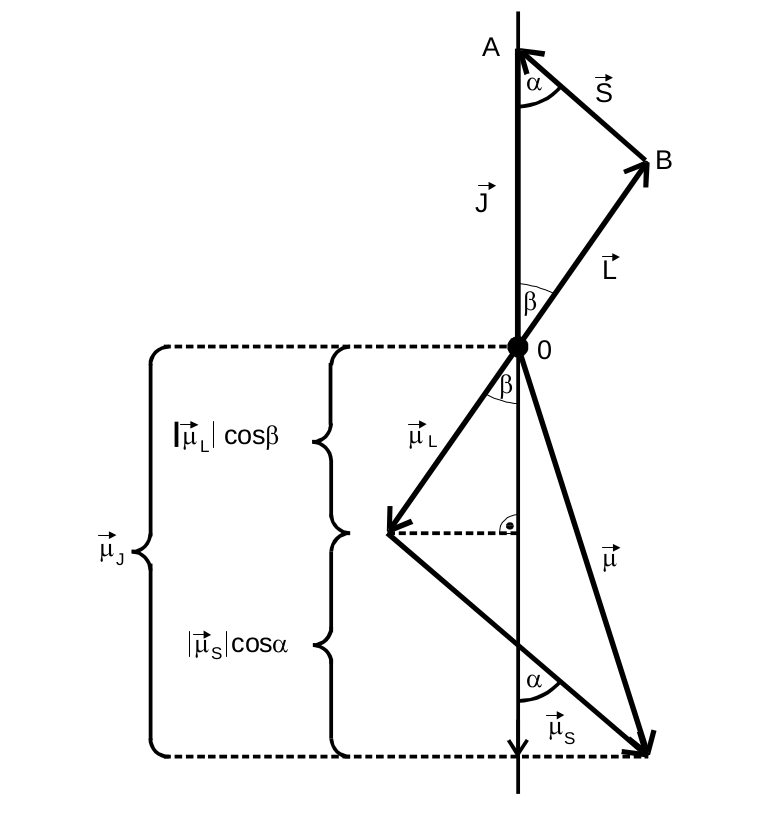
\includegraphics[width=0.55\textwidth]{../figures/vektor.png}
 \caption{Vektorielle Darstellung der magnetischen Momente und der Drehimpulse der Elektronenhülle.[Skript V606]}
 \label{fig:vektor}
\end{figure}

Mit einigen Umformungen und der Näherung aus der Quantenmechanik, dass $g_S \approx 2$ ist, vereinfacht sich Gleichung~\eqref{equ:mu_J1} zu
\begin{align}
  \label{equ:mu_J2}
  | \vec \mu_J | \approx \mu_B \sqrt{J(J+1)} \cdot \underbrace{\frac{3J(J+1) + (S(S+1)-L(L+1))}{2 J(J+1)}}_{g_J} \;
\end{align}
mit dem \emph{Landé-Faktor}
\begin{align}
  \label{equ:lande}
  g_J := \frac{3J(J+1) + (S(S+1)-L(L+1))}{2 J(J+1)} \; .
\end{align}

Ein weiteres Phänomen, das für die Berechnung von $\chi$ zu berücksichtigen ist, ist die \emph{Richtungsquantelung}. Sie folgt auch aus der Quantenmechanik und ihre Konsequenz ist, dass nur Winkel von $\vec\mu_J$ möglich sind, bei denen die z-Komponente $\mu_{J_z}$ in Richtung des externen Magnetfeldes ein ganzzahliges Vielfaches von $\mu_B g_J$ ist. Folglich gilt
\begin{align}
  \label{equ:quantelung}
  \mu_{J_z} = -\mu_B g_J m
\end{align}
mit der \emph{Orientierungsquantenzahl} $m$. Da der Betrag eines Vektors die Größe der einzelnen Komponenten beschränkt, gilt mit Gleichung~\eqref{equ:mu_J2}, dass
\begin{align*}
  |m| \leq J
\end{align*}
sein muss und damit genau $2J+1$ Einstellmöglichkeiten für den Winkel existieren. Nun ist es auch möglich ein Energieniveau in $2J+1$ Unterenergieniveaus aufzuspalten
\begin{align}
  \label{equ:Zeemann}
  E_m = -\vec \mu_J \cdot \vec B = \mu_{J_z}\cdot B = \mu_B g_J m \cdot B \; ,
\end{align}
was als \emph{Zeeman-Effekt} bezeichnet wird.
Die Magnetisierung $\vec M$ einer Substanz kann nun mit Hilfe dieser Unterenergieniveaus berechnet werden. Die Boltzmann-Verteilung gibt die Besetzungshäufigkeit $Z(E,T)$ eines Energieniveaus mit einer bestimmten Energie $E$ bei einer Temperatur $T$ an. Wird nun Gleichung~\eqref{equ:quantelung} über alle möglichen $m$ mit der zugehörigen Besetzungshäufigkeit summiert und durch die Gesamthäufigkeit aller möglichen Orientierungen geteilt, ergibt sich das gemittelte magnetische Moment. Der Betrag von $\vec M$ ist mit dem gemittelten magnetischen Moment über
\begin{align}
  M = \mu_0 N \bar \mu
\end{align}
verknüpft. Nach einigen Umformungen und Näherungen ergibt sich für die Suszeptibilität $\chi$:
\begin{align}
  \label{equ:sub_calc}
  \chi = \frac{\mu_0 \mu_B^2 g_J^2 N J(J+1)}{3k_B T} \; ,
\end{align}
mit $N$ als Anzahl der pro Volumeneinheit vorkommenden Momente, $k_B$ der Boltzmannkonstante und der Temperatur $T$. Es ist sofort zu erkennen, dass
\begin{align}
  \chi \propto \frac{1}{T}
\end{align}
ist, was als \emph{Curiesches Gesetz} des Paramagnetismus bekannt ist.\newpage

Der Paramagnetismus äußert sich besonders stark in den Atomen Seltener-Erden, da ihre Elektronenhüllen einen großen Drehimpuls aufweisen. Dies liegt an den 4f-Elektronen. Der Drehimpuls der anderen Elektronen ist abgesättigt und trägt daher nicht zum Gesamtdrehimpuls bei. Die Anordnung der Elektronen innerhalb der nicht gesättigten 4f-Schale wird durch die \emph{Hundschen Regeln} beschrieben:
\begin{itemize}
  \item Das Pauli-Prinzip bestimmt, wie sich die Einzelspins $\vec s_i$ zu dem maximalen Gesamtspin $\vec S = \sum{\vec s_i}$ kombinieren können.
  \item Der Gesamtbahndrehimpuls $\vec L = \sum{\vec l_i}$ ist die maximale Summe aus den Einzeldrehimpulsen $\vec l_i$, die weder das Pauli-Prinzip, noch die erste Regel verletzt.
  \item Wenn die Schale weniger als halb besetzt ist, ergibt sich für den Gesamtdrehimpuls $\vec J = \vec L - \vec S$, für eine mehr als die Hälfte gefüllte Schale hingegen $\vec J = \vec L + \vec S$.
\end{itemize}

\subsection{Messverfahren zur Bestimmung der magnetischen Suszeptibilität}\label{sec:messung}

Mit Hilfe einer Brückenschaltung ist es möglich die Suszeptibilität $\chi$ eines Stoffes zu messen. In Abbildung~\ref{fig:bruecke} ist eine geeignete Schaltung zu sehen.

\begin{figure}[H]
 \centering
 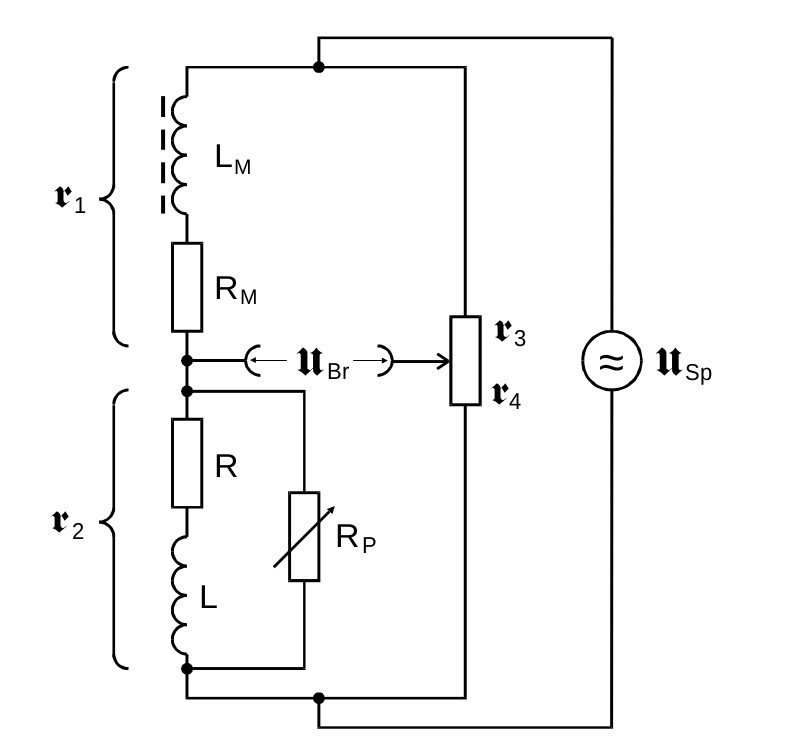
\includegraphics[width=0.55\textwidth]{../figures/bruecke.png}
 \caption{Brückenschaltung zur Messung der magnetischen Suszeptibilität.[Skript V606]}
 \label{fig:bruecke}
\end{figure}

Es werden zwei Spulen mit gleicher Induktivität benötigt, damit -- wenn eine der Spulen mit der auszumessenden Materie gefüllt wird -- die Induktivitätsdifferenz $\Delta L$ bestimmt werden kann. Da diese Differenz in der Praxis meist sehr gering ist, werden zwei möglichst identische Spulen benötigt, um eine hohe Auflösung für die Messung zu erreichen.

Es existieren zwei Methoden mit der in Abbildung~\ref{fig:bruecke} gezeigten Schaltung die Suszeptibilität zu bestimmen.
Zuerst wird die Brückenschaltung ohne Materie in den Spulen abgeglichen, d.h. die gemessene Brückenspannung $U_{\mathrm{Br}}$ wird durch die Widerstände auf den kleinst möglichen Wert eingestellt (theoretisch sollte keine Spannung mehr messbar sein).
Danach wird die Probe mit dem zu untersuchenden Material in einer der Spulen platziert und die neue Spannung gemessen. Bei hinreichend großen Frequenzen ($\omega^2 L^2 \ll R^2$) berechnet sich die Suszeptibilität nach
\begin{align}
  \label{equ:chi1}
  \chi(\omega \rightarrow \infty) = 4 \frac{F}{Q}\frac{U_{\mathrm{Br}}}{U_{\mathrm{Sp}}}
\end{align}
mit dem Querschnitt der Probe $Q$ dem Spulenquerschnitt $F$ und der Speisespannung $U_{\mathrm{Sp}}$.
Die zweite Methode besteht darin, dass nach dem einbringen der Probe nicht die Spannung gemessen, sondern der Widerstand am Potentiometer $R_3$ solange geändert wird, bis die Brückenschaltung erneut abgeglichen ist. Mit der Änderung des Widerstandes $\Delta R$ lässt sich nun die Suszeptibilität über
\begin{align}
  \label{equ:chi2}
  \chi = 2 \frac{\Delta R}{R_3}\frac{F}{Q}
\end{align}
berechnen.

\subsection{Unterdrückung von Störspannungen bei kleinen Signalspannungen}\label{sec:stoerung}
Bei Brückenschaltungen treten an den Ausgangsklemmen Störspannungen auf. Da die Brückenspannung sehr gering ist, können die Störspannungen diese nahezu vollkommen überdecken. Bei der hier vorliegenden monofrequenten Signalspannung kann dieses Problem folgendermaßen gelöst werden: Es wird ein Selektivverstärker benötigt, der wie ein elektronischer Filter wirkt und damit im Idealfall nur die monofrequente Signalspannung hindurchlässt. Die Wirksamkeit der Filterung hängt von der Güte $Q$ des Verstärkers ab: die Filterkurve (siehe Abb.~\ref{fig:glocke}) ist eine Glockenkurve deren Breite von der Güte beschrieben wird. Umso schmaler die Glockenkurve, desto besser die Unterdrückung der Störspannung. Daher ist auch klar, dass nicht alle Störspannungen vollkommen unterdrückt werden können. Des weiteren hat der Selektivverstärker den praktischen nutzen, dass er die geringe Brückenspannung verstärkt und sie somit leichter zu messen ist.

\begin{figure}[H]
 \centering
 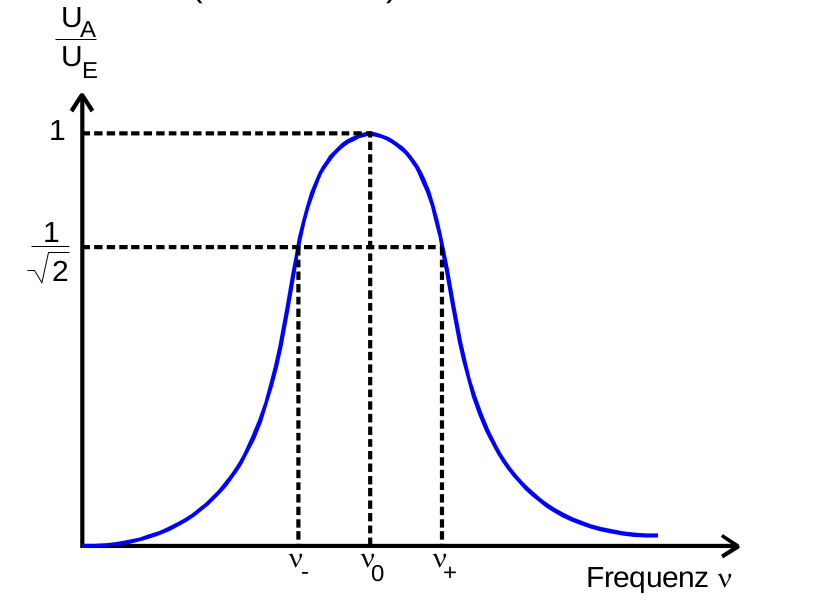
\includegraphics[width=0.4\textwidth]{../figures/glocke.png}
 \caption{Filterkurve eines Selektivverstärkers.[Skript V606]}
 \label{fig:glocke}
\end{figure}


%the end
